\newcommand{\comment}[1]{}

%\documentclass[a4paper,twocolumn,12pt]{article}

%\documentclass[a4wide,12pt]{report}

%\documentclass[a4wide,12pt]{article}
%\documentclass[informasjonssikkerhet]{gucmasterproject}
\documentclass[informationsecurity]{gucmasterproject}
%documentclass[gjovik]{gucmasterproject}

%\usepackage{pslatex} %% Doesn't seem to work - i.e. convert .eps to .pdf
 
\usepackage[utf8]{inputenc}     % For utf8 encoded .tex files
%\usepackage[latin1]{inputenc}
\usepackage[british]{babel}     % For chapter headings etc.
%\usepackage[pdftex]{graphicx}           % For inclusion of graphics

%From http://math.uib.no/it/tips/
   %% For grafikk
    \usepackage{ifpdf}
    \ifpdf
      \usepackage[pdftex]{graphicx}
      \usepackage{epstopdf}
    \else
      \usepackage[dvips]{graphicx}
    \fi
    %% Her kan du putte dine vanlige pakker og definisjoner

\usepackage{amsfonts}


%\usepackage[dvips]{hyperref}    % For cross references in pdf
\PassOptionsToPackage{hyphens}{url}\usepackage{hyperref}
\usepackage{mdwlist}
\usepackage{url}
\usepackage{here}

\def\UrlFont{\tt}

\begin{document}

\thesistitle{Specialization Report:\\ The Lightning Network}
\thesisauthor{Jardar Ton \\
jardart@stud.ntnu.no}
\thesisdate{\gucmasterthesisdate}
\useyear{2017}
\makefrontpages % make the frontpages
%\thesistitlepage % make the ordinary titlepage


\comment{
Front page - including
"   NTNU technical report front page including logos etc.
"   The text: "Specialization Report"
"   Title of project
"   Name of author and contact details
"   Date
"   Version

email address
"   MIS students must include "NISlab" as their affiliation.
Date:22.10.2003

Structure of Specialization Report
NTNU Gj\o{}ovik
}


\chapter*{Revision history}

\begin{center}
\begin{tabular}[H]{|l|p{35em}|}
\hline
Version \#  & Description of change (why, what where - a few sentences)\\
\hline
      0.1   & First version made available via Fronter\\
\hline
      0.2   & Corrected some spelling mistakes and added 'control questions' to Abstract, chapter 1 and 2\\
\hline
      0.2.1   & Removed the reference to a dead link in chapter 1 (keywords).\\
\hline
      0.2.1   & Replaced HIG logo by NTNU logo (just in case it is not done!) and removed references to information security\\
	\hline
\end{tabular}
\end{center}
\newpage

\begin{abstract}

\end{abstract}


\tableofcontents

%\chapter{Contents of the project description}
%The project description must use the gucmasterproject class file and contain the following elements/chapters:


\chapter{Introduction}

The lightning network(LN) builds on and improves the Bitcoin cryptocurrency technology. 
Since the first proposal of the Bitcoin technology in 2008\cite{nakamoto2008bitcoin} has the system and its technology been under constant development. It's popularity has spawned many alternate cryptocurrencies, but most relying on the same technology as Bitcoin. The Bitcoin network is a decentralized peer-to-peer network where every node has a copy of the distributed ledger called the blockchain. It contains information about every transaction done. No central authority need to verify new transactions; Cryptography and the distributed ledger makes the nodes in the network able to do so on their own.

\section{Transactions}
A transaction is what the name implies a transfer of money or value from one person to another. The book Mastering Bitcoin: Programming the Open Blockchain \cite{antonopoulos2017mastering} contains a detailed explanation of transactions which will be used for this section. Bitcoin is often explained in terms of actions or concepts such as addresses, wallets, senders and receivers, but these things are not really needed to explain Bitcoin transactions at its core. Transactions have two important elements: output and input. The input of a transaction is always the output of one or more other transactions. The output of a transaction can only be the input of one other transaction-i.e., a transaction output can only be spent once. There are two categories of transaction outputs: spent and unspent. The unspent transaction outputs are called UTXO, which the Bitcoin network keep track of. The UTXO require a cryptographic key to be used as input (spent), this requirement is placed by the creator of the transaction (previous spender). Bitcoins are "transferred" when Alice takes an UTXO she has the key to spend, creates a new transaction witch has the UTXO as input, has the same value as output but requires the private key of Bob to spend. This transaction is spread trough the network and since all UTXO is kept track of Bob can detect that he has the key to spend this UTXO.

\paragraph{}
The total output of a transaction must equal its total input. Similarly one whole UTXO must must be used as an input for a new transaction.
The flexibility comes from the possibility to have many inputs and outputs for one transaction.
Lets say Alice wishes to send Bob 5 coins, but she only has a 10 coin UTXO available. What she would do is to create a new transaction with the 10 coins as input, but having two outputs; One with 5 coins to herself and one with 5 coins to Bob.
This means that one can effectively split input values into smaller units. Several outputs can also be combined into one output by having many inputs and one output. 
This system of outputs being inputs in new transactions as shown in fig.\ref{fig:ln_trans} makes it possible to track a transaction output value by following this input output pattern in old transactions. The problem is that this investigation most likely will not be a single chain back to when the coins was created, but will show that the value has been split and mixed with other many times.


\begin{figure}[h]
    \centering
    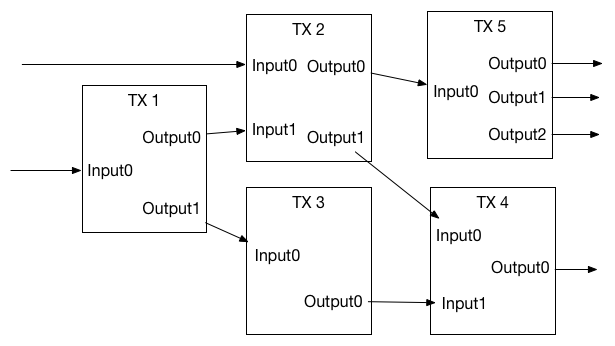
\includegraphics[width=10cm]{figs/LN_Trans.png}
    \caption{Visualization of transactions inputs and outputs. We can see the method of splitting founds by taking one input and splitting it out over many outputs. Similarly one can take many inputs from different transactions and combine them into one output.}
    \label{fig:ln_trans}
\end{figure}

\section{Blockchain}
The blockchain is the distributed data structure that stores all the transactions created. The same book Mastering Bitcoin: Programming the Open Blockchain \cite{antonopoulos2017mastering} also covers blocks and the blockchain well so it will be used as the source for this section as well. The structure consists of blocks where the transactions are stored and a reference to the previous block. This reference to the previous block is what makes it a chain as shown in fig.\ref{fig:blockchain} because we can follow the trail back to the genesis (first) block. The reference is the hash of the previous block and is stored in the header of the blocks. This header also contains among other things a timestamp, a merkle tree root, and a nonce. In addition to the headers the blocks contain many transactions.

\begin{figure}[h]
    \centering
    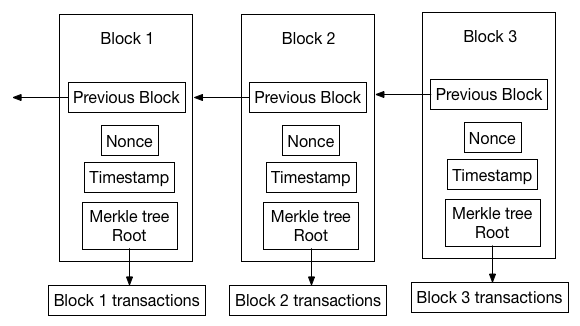
\includegraphics[width=10cm]{figs/blockchain.png}
    \caption{A part of the blockchain visualized. Each block contains a reference to the preceeding one.}
    \label{fig:blockchain}
\end{figure}


\paragraph{}
The merkle tree root in the header is a reference to the start of the a data structure in the block. The Merkle tree data structure is a binary tree, meaning each node at most has two children. It is used to summarize the transactions contained in the block; Making it effective to check if a transaction is included in the block or not. This type of structure is generated from the bottom up meaning the leaf nodes are created first. The transactions are all individually hashed and the resulting hashes are the leaf nodes. Then all the leaf nodes are hashed again in pairs of two and the result will be the parent node of the ones combined. This process of pairing two nodes together and hashing them to form their parent is done until there is only node left which will be the root of the tree. If a hash is the summary of its input then we can see how the root node would be the summary of all transactions in the block.

\paragraph{}
The timestamp in the header of the blocks tells us when a block was created. The creation process is called mining and consists of hashing the the newly created block header again and again while changing the nonce each time. The goal is to find a output of the hash function that starts with a specific number of zero's. Finding the nonce which gives this hash is very hard and requires a lot of computing power but verifying it once it has been found is very fast. Using all this computing power is called proof-of-work and is what gives the network its ability to have consensus about what transactions that have taken place. The blockchain can be considered one version of events or transactions that has taken place. This means that there could be several blockchains, each having a different version of what has transpired. The bitcoin network accepts the chain with the most amount of blocks in them as the valid one. This is because this chain will have the greatest amount of cpu-work invested in it, meaning to alter the events recorded in the blockhain the cpu-work needs to be redone creating a altered blockcain; It also needs to be performed so fast that the new chain becomes longer than the real one, thereby having the network accpenting the altered as the valid one.
Malicious actors would then need to have a more cpu-power than the rest of the network to influence the consensus.



\section{Scaling Problems}

One problem that has emerged with the popularity of Bitcon is its capability to scale well.
A paper called "On scaling decentralized blockchains"\cite{croman2016scaling} describes this problem clearly.
In the paper they define throughput as how many transactions that can be done each second, and latency is how long is takes for a transaction to be verified. Latency is influenced by the block creation interval, and throughput is influenced by two things: the size of the blocks and how often they are created. Having larger blocks means more transactions can be placed in each, and creating blocks faster will also make transactions be verified faster. While giving better throughput right now these solutions does not scale well. Blocks need time to propagate through the network; therefore large blocks created very often will cause problems. The paper does some observations about the limits of these two factors: with a 10 minute block creation interval, the blocks size should not be over 4MB; to reduce the latency the block creation interval needs to be reduced and therefore also the size, so for 80KB blocks the interval should not be less than 12 seconds.

\paragraph{}
One must also consider the size of the blockchain. At the time of writing this paper (October 2017) this is at about 138.000 MB or 134 GB \cite{blockchain_size}. While the storage capabilities on modern computers can accommodate this, the size of the blockchain in the future may cause users with standard consumer computer setup to not want to store the full blockchain because of the storage space requirements. Bitcoin users who have a updated copy of the blockchain run what is called a full node. SPV or simple payment verification nodes are a alternative that does not store the data, but asks full nodes for data when required. The storage requirement may cause many users to switch from a full node to a SPV node. 

\paragraph{}
The Lightning Network(LN) is a proposed solution to the scalability problems facing Bitcoin.
In the paper by Joseph Poon and Thaddeus Dryja \cite{poon2015bitcoin} warn that trying to scale the current system will lead to an extreme centralization in the Bitcoin network.
Having very large blocks, extreme difficulty mining, and a blockchain that has grown beyond a single hard disk will mean only people who can afford it, have the knowledge, and specialized equipment will be able to perform these tasks which where meant to be decentralized. The rest of the users will simply have to trust these central entities and one of the core aspects of the Bitcoin technology is lost.

\paragraph{}
The basic idea of the LN is that it allows two parities can exchange founds several times, and later only tell the rest of the Bitcoin network the final result.
When a exchange happens a new transaction with the current balance is created, but they defer telling the rest of the Bitcoin network about the transaction-i.e., the transaction being included in the blockchain. This means more exchanges can be done and the balance simply updated.
When one of the parties finally publishes it to the rest of the network it will be included in the blockchain and verified. Only one transaction needs to be published for the many that happened in private between the parties. These transactions happening without the blockchain knowing is why these are called off-chain transactions. This will reduce the amount of transactions needed to be published and therefore allow for more users and more transactions. But since many of those are off-chain it will not impact the Bitcoin network. The users connect to each other and use this method to route payment to each other creating a payment network which can scale independently from the blockchain.

\paragraph{}
Poon and Dryja. outlines several usecases in the paper \cite{poon2015bitcoin} where the LN has advantages or possibilities which the current Bitcoin solution does not. The first one is near instant payments, meaning a non-revocable transfer can be done in seconds. Micropayments becomes practical when avoiding the fees for having a transaction included in a block. Creating complex smart contracts outside the blockchain, these contracts are created by using advanced transaction scripts. Cross chain payment functionality between blockchains of different types could also be a possibility.


%%%%%%%% PAYMENT CHANNELS CHAPTER %%%%%%%%%%%%

\chapter{Payment Channels}

\cite{decker2015fast}

One of the core elements of the lighting network design outlined in the paper by Poon and Dryja \cite{poon2015bitcoin} is payment channels, which allow two parties to exchange founds between each other.
It is inside these that the balance between the parties in the channel are agreed on and updated.
The total amount of value in the channels is decided when the channel is created, and distributed to the parties according to the balance when something is published to the blockchain.


\section{Channel Creation}

The mechanisms for doing exchanges in the channel are simple themselves but there are many problems that arise when doing transactions off-chain.
A payment channel between Alice and Bob uses 2of2 multisignature Bitcoin transactions. A multisignature transaction means that multiple keys are required to spend output from a transaction. A 2of2 multisignature means that 2 keys of a potential 2 keys are required in this case-i.e., both Alice and Bob needs to use their keys. This ensures that both sides need to agree on transactions done with the coins in the channel. Without it, one of them could just create a new transaction spending all founds in the channel, publish it to the blockchain, and thereby stealing from the other.

\paragraph{}
To exchange founds in a channel one first needs to create whats called a "founding transaction". It's purpose is to create a common starting point for creation of new transactions in the channel. The input value of the founding transaction can come from one or both of the parties in the channel, but the output will have a 2of2 multisignature condition. Then a new transaction spending the output of the founding transaction is created which refund the input value of the founding transactions back to its original owner, also with a mutlisignature condition on it's output. At this point no signatures for either the founding or refund-transaction has been exchanged. This is done in a specific order where first the refund transaction is signed by both sides, and only then are signatures exchanged for the founding transaction. The reason for this is to avoid the founds being stuck in the founding transaction because of the multisignature condition on its output. If the founding transaction where published without or before a refund transaction was created, either Alice or Bob could render the founds unusable by not co-operating. After the signatures for the founding transactions has been exchanged it is published to the blockchain. The founding transaction starting point is now established; containing the total value available in the channel and allowing for refunds by either party by publishing the refund transaction.

\section{Channel operation}

The transactions describing the balance between Alice and Bob are called commitment transactions. Balance in the context of payment channels is how the total value of the channel will be split between the parties-e.g., if the total value of the channel is 10 coins and the balance is 5 to Alice and 5 to Bob; Alice decides to send Bob 1 coin; now the balance is 4 coins to Alice and 6 to Bob. This is shown in fig.\ref{fig:ln_commit} where we see the first commitment transaction on the left and the new on the right.

\begin{figure}[h]
    \centering
    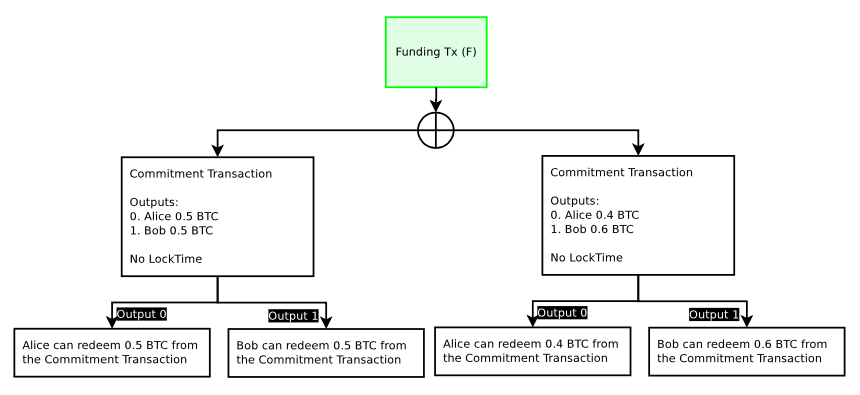
\includegraphics[width=12cm]{figs/ln_commit.png}
    \caption{The founding transaction is colored green to show it has been published to the blockchain. It has two commitment transactions. The leftmost is the original and the right shows the balance after Alice sends Bob 1 coin. Source: \cite{poon2015bitcoin}}
    \label{fig:ln_commit}
\end{figure}

The commitment transactions are all created from the output of the founding transaction just as the refund transaction was. The balance in the channel is described in the output data of these transactions, so these transactions takes the total value of the channel in the form of the output of the founding transaction and splits it between the parties in it's own output parameters. The refund transaction can be said to be the first commitment transaction since it describes the initial balance in the channel. This is the total value that was decided by the founding transaction, and the initial balance will be whatever each party contributed to the input of this. When the balance in the channel needs to be updated a new commitment transaction is created spending the output of the founding transaction again. The exchanging of founds between Alice and Bob consists of them creating new commitment transactions each time an exchange is done, which represents the new balance between the two. Alice and Bob exchanges signatures for each newly created commitment transaction to satisfy the multisgnature condition, which enables any one of them can publish it to the blockchain at any time they wish. A transaction output can only be spent once, so when a commitment transaction is published the founding transaction is spent, and all other commitment transactions created are useless. This means that the channel no longer has any uses, because its value or founding transaction is spent. So channels are closed out by publishing a commitment transaction. Therefore, to be able to do many exchanges between the sides in the channel the commitment transactions should not be published immediately. Only when something goes wrong, or both/one of the parties wishes the channel to close should the newest commitment transaction representing the current balance be published to the blockchain. 

\section{Trust and Revocation}

The payment channels should not require the parties to trust each other to be able to do exchanges between themselves.
As described earlier there are mechanisms that ensures co-operation such as multisignature addresses; makes malicious behaviour impossible such as rendering the founds unreachable with refund transaction in place. A mechanism is needed to solve the big problem of making sure only the newest commitment transaction which has the correct balance is published to the blockcain. Using the earlier example where a channel between Alice and Bob had the value of 10 coins and the balance was 5 to each. If Alice Does several payments to Bob and the balance ends up being 0 to Alice 10 to Bob, she could publish the commitment transaction where the balance was 5 to each and get all her money back. To deal with this problem it is proposed to penalize anyone who publishes any other commitment transaction than the latest. The penalty is that whoever published the old commitment transaction will loose all the founds the other person in the channel.
In order to punish the party who published an old commitment transaction it must be clear which one did it; known as the problem of ascribing blame. When the two parties exchanges signatures for a commitment transaction we end up with two different transactions. Bob signs one and sends it to Alice, and Alice signs one and sends it to Bob. This means both sides ends up with a half signed transaction which only needs their own signature before it is published to the blockchain. The multisignature requirement for commitment transactions means that each side can only publish the one they received from the other.
E.g., if Bob is the one who published a transaction we can find out, because he must publish one of those he received from Alice which already had her signature.

\paragraph{}
This is solved by revoking old commitment transactions. A transaction spending their own output of old commitments are signed and sent to the opposite party as an insurance. It means that one side will be able to spend the others output of old commitment transactions. In combination with enforcing a time period where the person who publishes commitment transactions cannot spend their output is the solution. So if Bob publishes an old commitment transaction Alice can detect this and spend Bobs output before he has the ability to spend it himself because of the timeout.

\paragraph{}
The timeout of transaction outputs or Revocable Sequence Maturity Contracts (RSMC) are the first step. When looking at the problem of ascribing blame there were two half signed copies of each commitment transaction; Bob got one where Alice has signed and Alice one where Bob has signed. Both of them are could be published to the blockchain but only one will, since they both spend the same output of the founding transaction. The timeout will be placed on the party who publishes the transaction; Reason being to try and steal from the other one would publish a transaction themselves-e.g., Alice publishes a old transaction where the balance in the channel favors her. For each set of commitment transactions each of them will have a RSMC on the output giving founds to the holder of the commitment transaction. The output which gives founds to the other party is not encumbered with this timeout. Fig.\ref{fig:ln_timeout} shows this structure with two sets of commitment transactions and their outputs. The timeout is enforced by confirmations of the commitment transaction. Confirmations is how deep a transaction is in the blockchain, so when a transaction is included in a block it has one confirmation, when another block is added to the chain it has two and so on\cite{antonopoulos2017mastering}. In the RSMC case it will make the person who publishes the commitment transaction unable to spend their output of that transaction until it has a set number of confirmations. In the paper they uses 1000 confirmations which will take some time when considering a 10 minute block interval.

\begin{figure}[h]
    \centering
    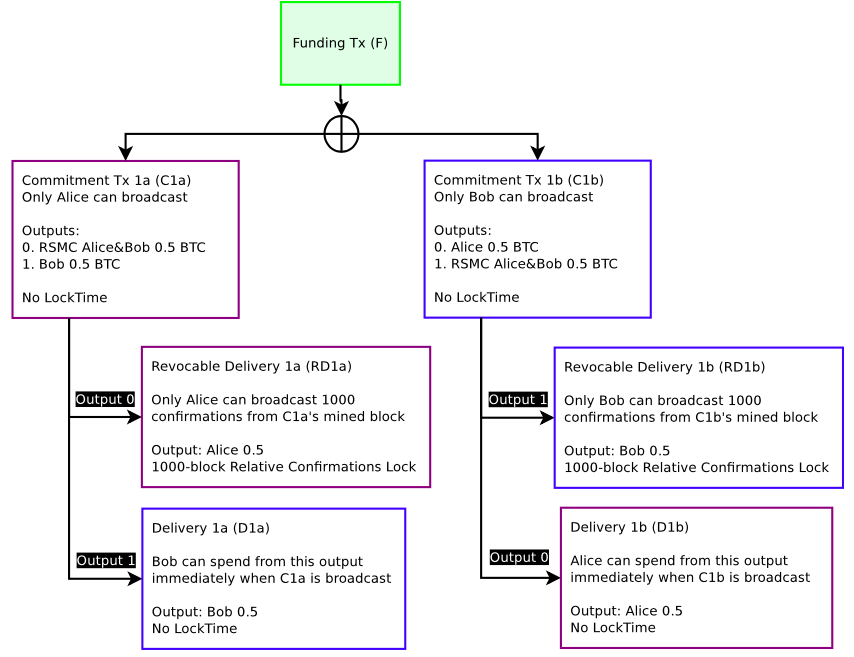
\includegraphics[width=12cm]{figs/ln_timeout.png}
    \caption{Here we see a pair of commitment transactions for Alice and Bob and their outputs. Purple indicates that Alice can publish and blue shows that Bob can publish. Source: \cite{poon2015bitcoin}}
    \label{fig:ln_timeout}
\end{figure}

The need to wait for confirmations to spend the output is something that is enforced on every set of created commitment transactions. It enables the next step that allows for old commitment transactions to be revoked. Whenever a new set of commitment transactions are created both parties sign and exchange whats called a Breach Remedy Transaction. This spends the output that is confirmation locked for that person-e.g., Alice creates a breach remedy transaction spending her output in the old commitment transaction and sends it to Bob. Now if either of the two parties publishes a old commitment transaction, they cannot spend their output at once because of the RSMC, and the other can publish the breach remedy transaction and get their output in addition to their own. The only for one of the parties to publish an old transaction and have the other party get all the funds is if the other party does not publish the breach remedy transaction in time. If enough time passes so that the commitment transaction gets enough confirmation the one who published it will be able to spend their output as long as the other party has not published the breach remedy transaction. Even so the other party still would get their output.

\paragraph{}
Lets say Alice and Bob has a channel with the value of 1 coin where they both contributed 0.5 coins each. They create a funding transaction, a refund transaction (which is really the first pair of commitment transactions paying back 0.5 coins to each), sign the refund transaction and then the founding transaction. After the funding transaction is published the channel is ready as shown in fig.\ref{fig:ln_breach}. The current commitment transaction (C1a for Alice and C1b for Bob) have their two outputs giving each 0.5 coins, one normal (D1b and D1b)   and one Revocable delivery (RD1a and RD1b) which needs confirmations to be broadcast. Then Alice sends Bob 0.1 coins. Bob creates his breach remedy (BR1b) which spends his 0.5 of the commitment transaction (C1b); this is the same 0.5 output that used in the Revocable delivery (RD1b).
Alice does the same thing and sends it to Bob. Now that the old commitment transactions (C1a and C1b) are revoked they can create the updated pair (C2a and C2b) witch the new balance which outputs 0.4 to Alice and 0.6 to Bob. Now Bob decides to broadcast the old commitment transaction (C1b) to the blockchain. A strange decision since in the old balance he has 0.1 coins less but it's still a violation of the agreement between the parties. 
He cannot claim Output 1 of 0.5 coins since he must wait for 1000 confirmations to do so because of the Revocable delivery (RD1b).
Alice sees on the blockchain that an old commitment transaction has been published. She has access to output 0 of 0.5 coins at once since it was Bob who published and therefore confirmation requirement for her. She also has the breach remedy transaction Bob sent her which spends output 1 of 0.5 coins. She can publish this before Bob because he has to wait for confirmations and thereby she gets both outputs and the total value of 1 coin.

\begin{figure}[h]
    \centering
    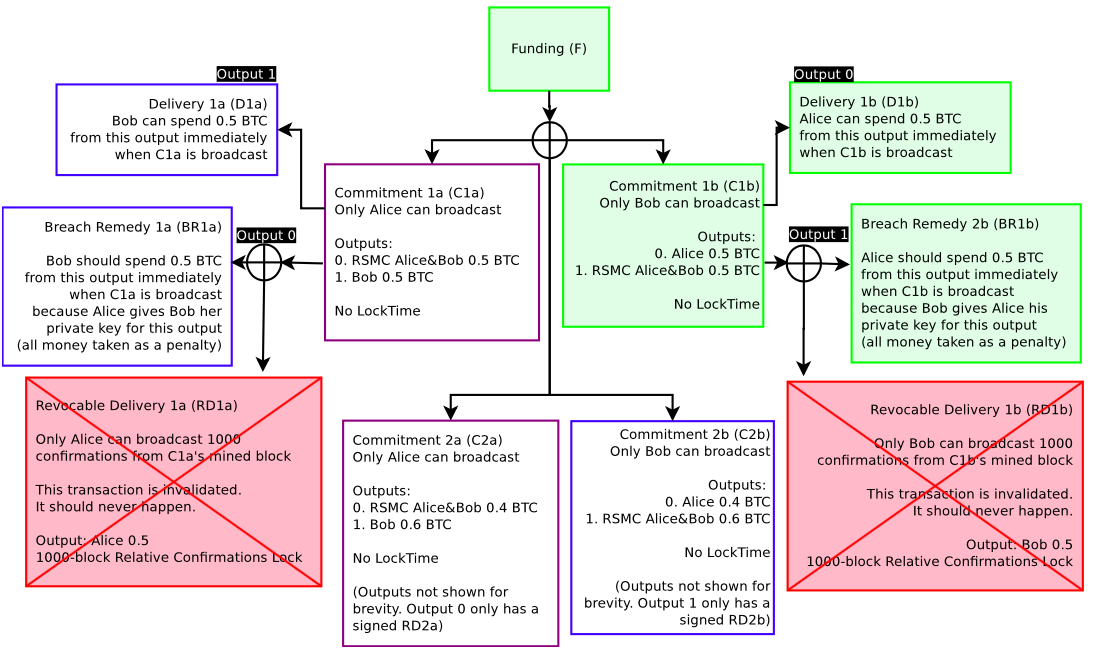
\includegraphics[width=14cm]{figs/ln_breach.png}
    \caption{This is what happens when an old commitment transaction is published. Green indicate that the transaction is published to the blockchain. We see two pairs of commitment transactions, with output transactions shown for the older pair. In this example Bob has published his old commitment transaction violating the agreement, therefore we see that Alice therefore can publish transactions spending both outputs.   Source: \cite{poon2015bitcoin}}
    \label{fig:ln_breach}
\end{figure}

Publishing a old commitment transaction as described above will spend the founding transaction and close the channel in addition to the other implications already described.
The channel can also be closed out by either of the parties publishing the most recent commitment transaction. If Bob was the one who published Alice can spend her output at once but Bob has to wait for confirmations in the blockchain before he can claim his. But still he will eventually get his output, and since no breach remedy transaction has been made since it is the newest commitment there is nothing Alice can do to stop him from getting his output.
The channel can also be cooperatively closed by both parties agreeing to do so. They simply create new transaction spending the founding transaction with the outputs reflecting the balance in the latest commitment. They echange signatures and it can be published on the blockchain. This transaction does not contain any Revocable delivery transaction on its output meaning both will be able to claim their founds at once. 
Another reason for doing this is that the total number of transactions that will be published to the blockchain will be less, one founding and one settlement instead of the extra revocation transaction.

\chapter{Networked Channels using HTLC}

The payment channels discussed in the previous section are for two parties to exchange founds with each other.
Poon and Dryja \cite{poon2015bitcoin} outlines a network of such payment channels forming
the Lighting Network. This means that a user can send founds to another across several payment channels. If everyone needed to create a payment channel everyone else it would not be very useful, so that is why networks of channels are used. Lets say Alice and Bob has a payment channel, but Bob and Dave also has one. Alice wishes to send founds to Dave and can do so by sending it first trough her existing channel with Bob, and Bob can use his channel with Dave to deliver him the payment.

\section{Hashed Timelock Contract}

As shown the payment channels used in the lighting network does not require trust to function. The same should be the case for doing payments across channels without trusting the intermediary nodes along the path. The mechanism that enables this is called Hashed Timelock Contracts (HTLC).
It works by creating contracts where intermediary nodes have a guarantee that they can get their money from the sender, if they first transfer to the receiver. By having the intermediary first pay the receiver and then get money from the sender one stops the intermediary from stealing the founds. If the intermediary was sent the founds first by the sender they could simply not pay the receiver and keep the money. But as mentioned for the intermediary to accept this they need to be sure that the sender will pay them what they have given the receiver. Using a hash function and an input or preimage R this guarantee can be crated. The receiver inputs R into the function and gets a hash H which is given to the sender. The sender promises to pay the intermediary if they can give R that generates H. The intermediary then promises to pay the receiver if they can provide a R that generates H. Since it was the receiver who created H and therefore has R they can give it to the intermediary and get the founds. Now the intermediary knows R and get the founds from the sender as promised.

\paragraph{}
The promise to pay someone in exchange for disclosing R is not just a promise. It is a transaction which needs R to be claimed. Therefore when the sender promises to pay the intermediary the sender is no longer in possession of the founds. So the founds are effectively transferred in a manner and direction one would expect (sender, intermediary, receiver) but requires R to be used. The timelock is what ensures that if no R is provided the founds can be returned to the one who promised them. It basically ensures delivery of the founds by setting a deadline on providing R. If no such thing existed the series of exchanges could be delayed or stopped by nodes not disclosing R and claiming their founds.
With and example and figures \ref{fig:htlc_promise} and \ref{fig:htlc_settle} illustrating we can see this in action.
Alice wishes to send founds to Dave, but to do so she must first send them through Bob and then Carol. Dave is the one who creates the hash H with the preimage R and sends H to Alice. She sees that there needs to be three transfers for the founds to reach Dave, so she creates the first HTLC with a three day timelock and sends it to Bob shown as step 1 in fig.\ref{fig:htlc_promise}. To re-iterate the HTLC is a transaction where the preimage R has to be given for the founds to be claimed, if R is not given within the timelock timeframe (three days in this case) the founds can be reclaimed by the creator of the HTLC. Bob creates a new HTLC for Carol with the same condition except that the timelock is two days shown as step 2 in fig.\ref{fig:htlc_promise}. In step 3 Carol creates a HTLC for Dave with the timelock set to one day. At this point the founds have been sendt but no one has claimed the founds in the HTLC's, and if it does not happen the founds will be returned when the timelock expires.

\begin{figure}[h]
    \centering
    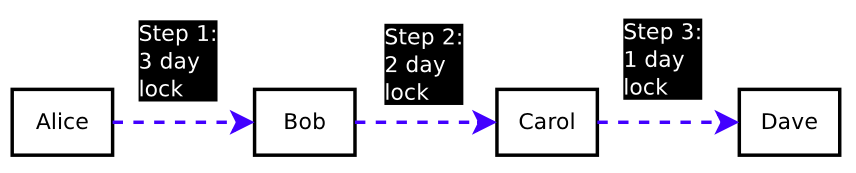
\includegraphics[width=11cm]{figs/htlc_promise.png}
    \caption{ Creating a HTLC between each node with a decrementing timelock. Source: \cite{poon2015bitcoin}}
    \label{fig:htlc_promise}
\end{figure}

In fig.\ref{fig:htlc_settle} we see steps 4, 5 and 6 done. Since it is Dave who knows R he must start the process. In step 4 he reveals R to Carol to claim the founds in their HTLC. Carol can then do the same with Bob in step 5, and finally step 6 where Bob can pull his founds from Alice.
Now the founds have been fully transferred from Alice to Dave.
The reason that the timelock must be shorter the closer we get to the final receiver of the founds is because it ensures that each person has time to pull the founds from the preceding one. Lets say that step 3 in fig.\ref{fig:htlc_promise} had a timelock of 5 days, and Dave waited 4 days to disclose R to Carol and get founds from her. The HTLC from Bob to Carol would have expired by then and Bob would have reclaimed his founds, meaning Carol has lost her founds to Dave without any way of getting them back.

\begin{figure}[h]
    \centering
    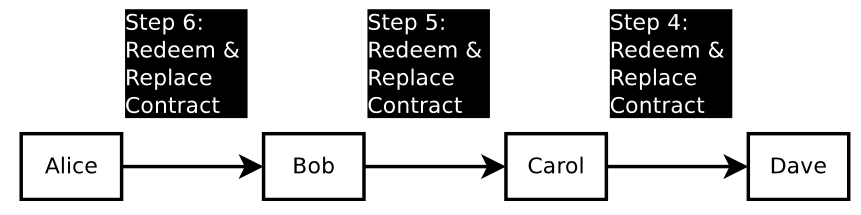
\includegraphics[width=11cm]{figs/htlc_settle.png}
    \caption{ Founds are pulled in reverse order meaning Dave the receiver gets the founds first and the sender Alice looses her's last. Source: \cite{poon2015bitcoin}}
    \label{fig:htlc_settle}
\end{figure}


\section{HTLC inside the payment channel}
The previous section explained how HTLC's can be used to transfer founds across different payment channels.
Here we will show how the HTLC construct interact with the already established dynamic within a payment channel.
A HTLC inside a payment channel will be a output of commitment transactions. Outputs of these commitment transactions reflected the balance between the parties inside the channel, so by having another output we can also reflect founds in transit. The HTLC output is a special type of output; it is a output script which can two different paths to redeeming the output: one is by providing the preimage R, and the other is by waiting for the timelock to expire. As with other output it can only be spent once, and this type must be spent in one of the two ways explained.

\paragraph{}
As an output of commitment transaction the HTLC uses founds available in the channel. If the value of a channel is 10 coins with a 5 to each split, a HTLC for 1 coin will be reflected in the commitment trasaction as the sender having 4 coins, but the total value of the channel will still be 10 (4 sender, 1 HTLC, and 5 reciver). If they both agree on who can spend the HTLC output-e.g., receiver knows the preimage R they can spend. or the timelock is over the sender can spend it, then they can cancel the HTLC and create a new commitment transaction reflecting the new balance. This new balance is either the receiver getting the value of the HTLC or the sender getting it back. This is how HTLC's are resolved off-chain.

\paragraph{}
The two ways of spending a HTLC output by creating a "delivery" transaction which needs the preimage R to be valid and the "timeout" transaction which is not valid until the timelock is gone. If they fulfill their conditions both of these can be broadcast to the blockchain. But since the these transactions spend a output of a commitment transaction the commitment transaction would also need to be broadcast on the blockchain to be able to spend its outputs in new transactions. As explained earlier both parties have the opportunity to broadcast their commitment transaction but restrictions will apply when doing so. The one who published a commitment transaction had to wait before being able to claim their output, while the other party could claim theirs at once. In addition, if the commitment transaction was old and had been revoked by the creation of a superseding transaction spending the
broadcasters output, the other party could use this to get all the founds since the broadcaster had to wait to spend their output.
Similar mechanisms are used when adding the third HTLC output on the commitment transactions. Using the example of Alice and Bob having a 1 coin channel with a 0.5 to each balance we can see how this works. Alice sends Bob 0.1 coins using a HTLC and they create a new pair of commitment transactions (C2a, C2b) as shown in fig.\ref{fig:htlc_commit} where Alice can broadcast the purple ones and Bob the blue.


\begin{figure}[h]
    \centering
    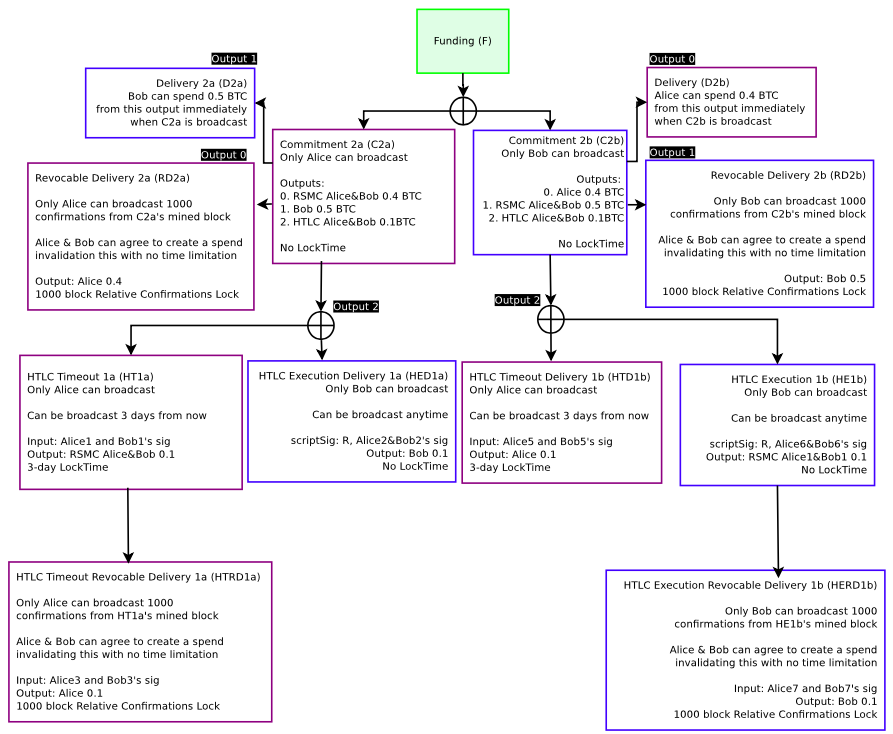
\includegraphics[width=14cm]{figs/ln_htlc.png}
    \caption{ Overview of transactions when including HTLC output to the commitment transactions. Again we have a mirrored structure with the left side showing the case of Alice broadcasting the commitment and the right side Bob broadcasting.  Source: \cite{poon2015bitcoin}}
    \label{fig:htlc_commit}
\end{figure}


\paragraph{}
If the sender, in this case Alice is the one who broadcasts her commitment transaction (C2a) she will have the restrictions placed on her.
In fig.\ref{fig:htlc_commit} this means that the left side will be executed. The commitment transaction (C2a) has three outputs: output 0 is 0.4 to Alice herself (RD2a), but since it is her commitment transaction she will have to wait for confirmations to be able to spend; output 1 is 0.5 for Bob which he can spend immediately (D2a); output 2 is the HTLC which has two different output paths, Bob can spend at once creating a transaction containing the preimage R (HED1a), or Alice can spend (HT1a) when the timelock has expired but this spend will a RSMC (HTRD1a) having her wait for confirmations similarly as her normal output. This is because similarly as old commitment transactions are invalidated by exchanging breach remedy transactions the same is done by exchanging keys for spending the HTLC output. So if an old commitment transaction is broadcast the party who broadcast will also loose the HTLC output in addition to the normal output, since the other party will be able to spend it and broadcast to the blockchain before the RSMC has enough confirmations. In this case it will enable Bob to broadcast a transaction spending the value of the HTLC before Alice can.

\paragraph{}
In the case of Bob, the receiver broadcasting the commitment transction (C2b) the left side of fig.\ref{fig:htlc_commit} will be executed. We can see that the structure is the same but now Alice and Bob have different restrictions. The output of the commitment transactions remains the same except that now it is Bob who has to wait for confirmations to get his normal output of 0.4 because of the RSMC (RD2b), and Alice can spend hers at once (D2b). In the case of the HTLC output the two parties still have their sender and receiver status meaning Alice can only spend by Timeout of the timelock (HTD1b), and Bob only by providing the preimage R (HE1b). However, since it now was Bob who broadcasted the commitment he is the one who has to get restricted getting the output. So the output of the transaction spending the HTLC output using R (HE1b) is now a RSMC (HERD1b) which will require confirmations to become valid. This is to once again enable the other party (Alice) to get the value in the HTLC if the commitment transaction is an old one.  

\paragraph{}
Similarly as with channel operation without HTLC it is desirable to avoid publishing to the blockchain unless it is necessary. The parties can cooperate and agree on new commitment transactions with or without HTLC outputs. To resolve a HTLC one of the parties must simply prove to the other that they are capable of spending the HTLC output and can do so on the blockchain if they wish. If Bob is the receiver he can publish the commitment transaction and if he has the preimage R he can also create a transaction spending this; because he is the broadcaster he must wait for confirmations on both but will eventually receive his founds. If Bob does not have the preimage R and the timelock has expired Alice can do the same. Since they can prove to the other party that they have this possibility they can instead just create a new commitment transaction pair with the HTLC value either transferred to Bob or returned to Alice, thereby keeping the channel open. When doing this they need to invalidate their old commitment transactions and also the HTLC output to these by exchanging breach remedy transactions and keys. So again we have a system for exchanges between two parties but with the possibility of also using HTLC's which requires no trust, few transactions to be broadcast to the blockchain unless one party is unresponsive or unwilling to co-operate, and allows for founds to be transferred trough many channels.  
When using the HTLC construct to send founds across these channels as shown in fig.\ref{fig:htlc_settle} broadcasting to the blockchain as discussed in this section will ensure the transfer will finish in the event of a node not co-operating as illustrated in fig.\ref{fig:htlc_bc}.

\begin{figure}[h]
    \centering
    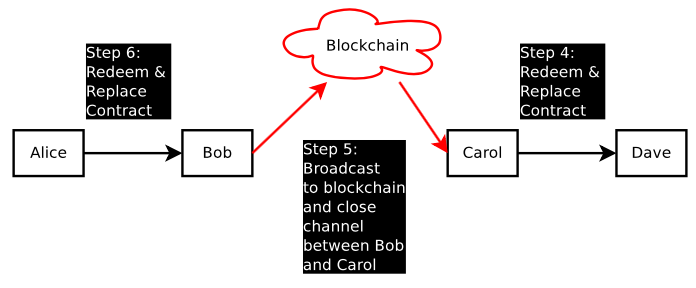
\includegraphics[width=10cm]{figs/htlc_bc.png}
    \caption{ Settlement of HTLC contracts in the event of unresponsive node. Source: \cite{poon2015bitcoin}}
    \label{fig:htlc_bc}
\end{figure}

%%%%%% NO BLANK PAGES 
%\let\cleardoublepage\clearpage

\chapter{Implementation of LN}

Since the LN paper was published \cite{poon2015bitcoin} there has been ongoing work to implement the technology\cite{LN_imp1}\cite{LN_imp2}\cite{LN_imp3} and also to create a specification called BOLT (Basic of Lightning Technologies) \cite{LN_spec}. In 2015 one of the authors of the LN paper Dryja outlines several things that must happen to make the LN work with Bitcoin \cite{SB_bip}. Timelocks, transaction malleability, and allowing spends to be created from unsigned transaction.
The latter being needed when creating and signing the refund transaction before the founding transaction when a channel is created.




\section{Segregated witness}
Segregated Witness or segwit is a upgrade to the Bitocoin technology first presented at the 2015 Scaling Bitcoin conference\cite{SB_segwit}. The upgrade changes how transactions are validated and how the transactions themselves are structured.
In chapter 1 we discussed how transactions consists of inputs and outputs. A requirement was placed on the output to be able to spend it which was a cryptographic key. But we have also seen other conditions that must be fulfilled to spend such as multiple signatures or a timelock. These conditions to spend a output is called "locking-script", "witness-script", or scriptPubKey \cite{antonopoulos2017mastering}. It is called a script because output conditions can be "scripted" to require specific things. The witness-script is included in the output section of each transaction. Similarly the input section of transactions have a script called "unlocking-script", "witness" or scriptSig. The witness fulfills the conditions created in the output which the input spends. So we have transactions with output scripts that sets conditions to spend, and the transactions spending these outputs have input scripts that meets these. The idea of segwit is to separate the witness or unlocking script from the transaction into a separate data entity. 

\paragraph{}
There are many reasons and benefits of doing this seperation\cite{antonopoulos2017mastering}\cite{BC_segwit}. One of these is that it disables transaction malleability. The bitcoin transactions have a transaction id (txid) which is a hash of all its properites including the scriptSig or witness. The malleable parts of a transaction is the scriptSig, this is because a transaction is unique and founds can only be spent once; so if the choice of inputs, choice of outputs, or the value of these changes, it is no longer the same transaction.
Therefore, when the transaction has been created most of it is non malleable. But the scriptSig can be modified in different ways without invalidating the transaction and without knowing the public key \cite{BIP62}. Since a hash function is used to create the txid it will result in the transaction having a completely different id. With segwit the txid is created without the scriptSig since it is locate in separate data structure meaning the txid will be immutable once it is created. Another very important benefit is that the size of transactions are smaller since it no longer includes the scriptSig. The witness data structure can be deleted after it is verified or simply do not need to accompany the transaction at all-e.g., Simple payment verification (SPV) do not need the witness data.
Other improvements are reduced computational requirements for the script operations which will lead to faster verification of scritSig's.
There is also script versioning to make it easier to introduce new operations without running into problems with nodes supporting them or not.

\paragraph{}
The segwit upgrade is now active on the Bitcoin network because a majority of the nodes do support it. This type of change is whats called a soft fork. A fork is when the blockchain split and diverges \cite{antonopoulos2017mastering}. A change or upgrade in how the nodes operate in the network can cause a fork since the nodes who upgrade will only follow the new rules, and the non upgraded nodes will only follow theirs. If the new and old rules are incompatible, the result will be a split blockchain, each with a set of nodes working only with their own methods. This is known as a hard fork and is undesirable because it will split the network if not everyone upgrades or decided to use the new consensus rules. A soft for as the segwit upgrade was does not cause a fork at all, but allows the upgraded and ungraded nodes to work together-i.e., the upgrade is backwards compatible. When a non segwit supported node looks at a segwit transaction output it will interpret it as being spendable by using an empty signature, but the transaction will still be considered valid \cite{antonopoulos2017mastering}. Segwit enabled nodes which is the majority, will be able to look at the witness and validate transactions correctly. Therefore, segwit transactions are backwards compatible because they will not be invalidated by old non segwit nodes.

\paragraph{}
The activation of segwit is important for the LN. As described above one of the issues segwit fixes is the transaction malleability problem, which in the Lightning Netowrk paper \cite{poon2015bitcoin} is stated as essential for the design outlined to work properly. The issue outlined there is destroying signatures such that transactions are no longer valid. A issue outlined in the LN Community Blog Post\cite{LN_segwit} about the alpha release of their LN implementation is monitoring of the blockchain. The two parties in a channel had to monitor the blockchain for the other broadcasting old commitment transactions. With segwit the transaction id can be known ahead of time because it cannot be changed once a transaction is crated. This also creates the possibility for outsourcing the blockchain monitoring to a third party, meaning the Lightning nodes does not need to be a full Bitcoin node.

\chapter{Networking and Routing}

The LN consists of people having payment channels open to each other, thereby creating a network of channels. The topology of the network will impact other areas such as routing, centralization, optimization, and privacy.  As we have seen in the previous chapters a channel will have a value which is decided in the founding transaction of the channel. This means that  the founds is tied to this channel and cannot be used for something else. The founds will only be available to use for other purposes by closing out the channel. The transfer capacity of a channel will be dependent on the total value of the channel, meaning a channel cannot transfer more than the total value simultaneously. Because of these inconveniences of keeping payment channels available for other people to transfer founds the LN paper\cite{poon2015bitcoin} proposes that one should pay fees to the intermediary nodes for transferring founds. 

\section{Topology}
The LN paper itself\cite{poon2015bitcoin} imagines that eventually the network will mainly consist of core nodes which maintain open channels with each other, while average users will connect to these when needing to do transfers. This topology is called hub-and-spoke, where the core nodes are the hubs and the spokes are the end users connecting to the hub. These core nodes will have the resources to run channels with high capacity for long periods to other core nodes. The fees end users pay for transferring founds will be the incentive for running these, core nodes effectively providing a payment transferring service to end users. 

\paragraph{}
A important aspect of the hub-and-spoke topology to which degree anyone can become a hub.
A paper discussing payment channel networks\cite{mccorry2016towards} refers to this a the open-memberhip property.
This is decided by the requirements for becoming a hub. 
If they are too high only entities with enough resources will be able to run hubs potentially resulting in more centralization.
But if there are no requrements and anyone can become a hub there can be more challenges in regards to routing as discussed in the next section. The problem of the open-membership property is somewhat of a similar problem discussed in chapter one where trying to scale Bitcoin on-chain can lead to very high requirements to run a full-node that processes transactions. 

\paragraph{}
The degree of decentralization possible in the network has sparked some debate. Some argue that a fully decentralized solution might not be likely \cite{sceptic1}, and some even that the only outcome can be a few central "banking" hubs\cite{sceptic2}. Most of the arguments made against the possibility of a decentralized solution is related to requirements of participating in a fully decentralized network. There is the notion that there will be a trade-off between high connectivity in the network with each node having multiple channels open with other node, and path length of payments meaning the number of nodes involved in routing a payment. If nodes have high connectivity there is greater possibility of shorter paths existing, and if the connectivity is low the average path length might be longer.
The arguments based on this notion is  that having high connectivity is not feasible because the founds will be spread in many channels locking them there and the value in each channel will be small. Similarly, long paths is also unpractical because it will tie up more total founds per transaction-i.e., the transferring mechanism with HTLC requires each node to "lend" the sum forward to the next node and later reclaim the same sum from the preceding node; meaning the while a payment is happening it ties up part of the capacity in the channel, and the more nodes and therefore channels being used per payment the more total founds are being temporarily made unavailable.
In addition if a larger payment needs to be routed it can cause additional issues such as finding a path where all channels have enough capacity to route it.

\paragraph{}
There also has people arguing against the claims about the impossibility of decentralization in the LN \cite{answer1}\cite{answer2}.
Here it is argued that the notion of nodes "lending" founds forward is with the HTLC construction is wrong.
Instead the nodes receive balance in one channel and loses it in another effectively trading balance-e.g., Alice receives a HTLC from Bob, she creates a HTLC with Carol; in the Bob-Alice channel Alice will gain founds and in the Alice-Carol channel she will loose founds.
Also, a LN payment of creating HTLC's and resolving these by pulling the founds will happen in milliseconds so that the founds will not be tied up inside the payment channels to any large degree. It is also pointed out that the LN is a scalability solution for micro-payments and low value payments so channel capacity for large payments should not be considered a problem. As both \cite{sceptic2} and \cite{answer1} agrees on that if just a single payment is to be made it is in no way beneficial to use the LN as it will require two transaction (founding and closing) to do the transfer, while doing it on-chain will only require one.


\section{Routing}
A paper by Prihodko et al. where a routing algorithm called Flare\cite{prihodko2016flare} is suggested, also discusses current suggestions for routing. 
They state that in regards to the hub-and-spoke network with enforced roles, meaning where some nodes can only route payments (the hubs) and others only send or receive payments; the strong separation means that the set of hubs will be known and also not constantly changing. Therefore finding a route to a specific hub will be easy, because all important nodes and routes between them will be known.
They also note some negative aspects with this; like 
end user nodes not having any reason for staying connected to the network, and therefore payments might not reach recipient at once since they will need to connect to the network first.
It can also cause some high degree of centralization in the network as mentioned before and this will also decrease the fault tolerance.

\paragraph{}
The  same paper by Prihodko et al.\cite{prihodko2016flare} also covers two other suggestions which are quite similar.
They where both originally discussed on the LN developer mailing list\cite{rusty_routing1} \cite{rusty_routing2} \cite{rusty_routing3}. The concept is that a subset of hubs will be selected at random to become global "beacons". The other nodes find the paths to these, meaning the beacons will act as meeting place between sender and receiver. The receiver will know its paths to the beacons and therefore pick the best one and send it to the sender. Now the sender knows the path from a beacon to the sender and they already know their paths to the beacons. The task of being beacons will be rotated at intervals to make it harder for a single entity to control parts of the network. Becoming a beacon will mean that a lot of traffic will be coming but also earnings from fees will high.
Prihodko et al. points out several challenges with this strategy: the requirements for being a beacon is so high that the list of potential beacons would be too small; beacons themselves could be targets of DOS attacks; the channels crated while a node is a beacon will have very limited use afterwards. The other suggested solution is very similar and also uses beacons but these are personal for each node. Nodes will then have find similarities in their beacons to do transactions. A solution where each node can become one of the beacon nodes for other nodes the result will be a more evenly used network where nodes have incentives to stay online and connected.

\paragraph{}
The flare protocol by Prihodko et al.\cite{prihodko2016flare} is a proposed routing protocol for the LN. It uses source routing, which means that the sender or source of the message will be in control of selecting the route. In routing protocols that does not use source routing the intermediary nodes are responsive for finding a route that gets the message in the right direction. The reason source routing should be used in the LN is because it gives the sender control, which they need for several reasons\cite{prihodko2016flare}: it enables privacy because it helps onion routing, since the user is the only one who should knows the full route\cite{SB_onion}\cite{LN_onion_implementation}; the sender of a payment will be the one paying the fees to the intermediary nodes, and they should therefore be able to predict the cost of using different routes. With flare each nodes proactively gathers information about the topology and stores it in a routing table. This is gathered by using local neighbour nodes and a set of random beacon nodes to get a more global view. A sender node also does reactive information gathering when a payment is done. The sender and receiver compare their routing tables to find suitable routes; then information about route length, fee cost, and route capacity is used to choose a path. 

\chapter{Onion Routing}

Onion routing is a mechanism that provides anonymity when messages are routed inside a network. 
Specifically relationship anonymity which is the concept of unlinkability between the sender and receiver of a message \cite{pfitzmann2001anonymity}. For a message the sender might be known by some, and for others the receiver can be known, but to link the sender and receiver together as having exchnged the message should be impossible. This is a feature that has been suggested for the LN \cite{LNDM_onion}\cite{SB_onion} and also have a implementation under development \cite{LN_onion_implementation}.

\section{Mixing and onions}

Something similar to onion routing, later known as a mix network was proposed by Chaum in 1981 \cite{chaum1981untraceable}.
The system he suggested provided relationship anonymity and hid the content of the communication. The system consisted of intermediary mix nodes between the sender and receiver which accepted encrypted messages, decrypted them and then forwarded them. Since the messages was encrypted when they arrived and decrypted when they left the mix node it was impossible link the incoming message to a outgoing one for a observer. In addition this done in batches to avoid timing information being used to identify messages. This meant that a observer monitoring the network would not be able to trace a message from its origin to its destination because it was mixed with many other messages.

\paragraph{}
Onion routing was first proposed by Goldschlag et al. in a paper titled "Hiding Routing Information" \cite{goldschlag1996hiding}.
The mechanism they suggest is similar to to the one proposed by Chaum \cite{chaum1981untraceable}, but their goal is to construct a more general solution for different communication requirements, and not just a anonymous mail delivery solution as Chaum had done. They wanted a real time, anonymous, and bidirectional socket connection between two parties who wish to communicate. The term "onion routing" refers to the layered construction of the messages used in the solution. In the center of the onion there is the payload of the message, each layer on top of the center is encrypted routing information. When message is sent a path to the sender is selected, and for each intermediary node in the path a layer is constructed telling that particular node where to send the message next. Each layer is encrypted such as the node the layer is intended for can decrypt it. So, this results in each node in path only knowing where they received the onion from, and after they decrypt the top layer, where they should forward the onion to. Relationship anonymity is established since none of the nodes can know both sender and receiver. A node or onion router can also be part several different paths meaning the messages can be somewhat mixed in a similar manner as a mixing network.
A series of papers refining the idea of onion routing was published after the original one which resulted in the creation of a well known onion routing network Tor \cite{reed1998anonymous}\cite{goldschlag1999onion}\cite{dingledine2004tor}.

\paragraph{}
According to one of the authors who contributed to all the onion routing papers previously mentioned Paul Syverson the concept of a mix network (mixnet) and onion routing network is often confused \cite{syverson2009m}.
A big similarity is that both a onion routing network and a decryption mixnet have multiple layers of encryption which is removed as the message is routed through the network.
But according to Syverson one of the main difference is how they achieve their security which allows for anonymity. 
A mixnet relies mainly on mixing while a onion routing network will use unpredictable paths. The threat model of the mixnet is that an adversary can observe traffic everywhere in the network and therefore the security must come from heavily mixing the messages. Onion routing that uses unpredictable paths which are difficult for a adversary to observe because the adversary will have limited monitoring capabilities. But if a adversary can observe traffic in both ends of a path in a onion routing network the anonymity provided would be minimal, because the traffic could be recognized. To recognize the traffic several places in a mixnet would in comparison be extremely hard. Again, to reiterate that the intended use for the two methods are also different. Mixnets are generally for unidirectional and high latency traffic, while onion routing is for low latency bidirectional traffic.


\section{Sphinx}

Sphinx \cite{danezis2009sphinx} is a packet format originally intended for anonymous messages within a mixnet, but using it for onion routing within the LN has been suggested \cite{LNDM_onion} \cite{SB_onion} and also implemented \cite{LN_onion_implementation}.
Sphinx has bitwise unlinkability which means that the bit pattern of a message entering a node (mix) should not be linkable with the bit pattern of the message when it leaves the mix. It supports paths (routes) lengths of long as the sender wants, meaning there is no limit to how many mix routers a message path can consist of. Also Sphinx has countermeasures to to "tagging attacks", which is when a message is tagged by modifying it and replayed. Finally, it is very compact compared to other cryptographic message formats, and also compared to earlier proposals of formats to use for onion routing in LN \cite{LNDM_onion}.

\paragraph{}
What allows for such a compact and small message format is how the key distribution are handled. As with other onion routing and mixing solutions, the sender encrypts a message with one layer per node in the path of the message. For the sender to encrypt and the nodes to decrypt, the sender and each node needs to establish a shared key. This is because each node in the path should only be able to decrypt their layer and find out where to send the message to next and nothing more. The shared key between the sender and each node must also be available when the message is created for the user to be able to encrypt the layers.
Sphinx uses the Diffie Hellman key exchange (DH) \cite{diffie1976new} which allows two parties to establish a common shared key over an unsafe channel. 
To do this they need a finite cyclic group $G$ of prime order $q$ with a generator $g$. The order $q$ denotes how many elements are contained in $G$ and if $q$ is prime the group is cyclic. The generator $g$ can be used to generate all elements in $G$ as such: every $e\in G$ can be generated by $e=g^i$ with some $i$. All elements created in the key exchange by using $g$ should be in the group $G$ and therefore the $i$ chosen should be $1 \leq i < q$, or in other notation: $i \in _R \mathbb{Z}_q^*$ \cite{algebra}. Here is how Alice and Bob generate a shared secret $S$:

\begin{itemize}
    \item Alice chooses her secret $a \in _R \mathbb{Z}_q^*$, generates A and sends it to Bob:  $A\in G, A = g^a  $
    \item Bob chooses his secret $b \in _R \mathbb{Z}_q^*$, generates B and sends to Alice:  $ B\in G, B = g^b$
    \item Alice calculates shared secret using B from Bob and her secret a: $ S \in G, S = B^a $
    \item Bob calculates shared secret using A from Alice and his secret b: $ S \in G, S = A^b $
\end{itemize}

\noindent In Sphinx \cite{danezis2009sphinx} nodes has a private key $x_{n} \in_R \mathbb{Z}_q^*$ which is their secret exponent in DH key exchange. A corresponding public key $y_{n} \in G$ is created using the the generator $g$ of $G$ and the private key like this: $y_{n} = g^x_{n}$. The public key $y_{n}$ is available for everyone and thus the sender can use it to generate the shared secret when creating the message. The sender chooses their secret exponent $x$ and uses the generator to create a element $\alpha$ in the group $G$:
$\alpha \in G, \alpha = g^x$. Now the sender can use the public key $y_{n}$ of the node with their own secret exponent $x$ and create $s$ the shared key: $s = y_{n}^x$. This shared key is used to encrypt the layer intended for that node. The $\alpha$ element generated by the sender is included in the header of the message without any encryption as it is used by the node to generate the shared secret $s$ by using its private key $x_n$ like so: $s = \alpha^{x_n}$. Now the node can decrypt the rest of the message and forward the message.

\paragraph{}
Using the method outlined above the sender would need to generate a different $\alpha$ element for each node in the path.
Each one of those would also need to be included in the message such that every node can calculate their shared key.
To save space the same $\alpha$ can be used for every node in the path meaning only one $\alpha$ would need to be included in the message. Remember each user will derive the shared key by using their private key $s = \alpha^{x_n}$, meaning the same $\alpha$ value will result in different shared keys $s$ as long as the nodes private key $x_n$ is different. But having the same $\alpha$ value for a message would mean that this message would become linkable with itself. If different values where used for each node this would not be a problem as the value would change for each hop, but having a unencrypted constant value will make the message recognizable. Sphinx solves this by a technique called blinding which mutates the element $\alpha$ for each hop. Each node calculates a blinding factor $b$ using a hash function $h_b$ with their $\alpha$ and shared key $s$ as input, and uses it create the $\alpha$ for the next node. Of course this means that the sender must also calculate the blinding factor when creating the message.

\paragraph{}
The sender selects a path containing $v$ nodes meaning $ \{\alpha_0, \alpha_1,...,\alpha_{v-1}\} $ group elements, $ \{s_0, s_1,...,s_{v-1}\} $ shared keys, and $ \{b_0, b_1,...,b_{v-1}\} $ blinding factors are be created \cite{danezis2009sphinx}: \\
$\alpha_0 = g^x, s_0 = y_{n_0}^x, b_0 = h_b(\alpha_0, s_0)$ \\
$\alpha_1 = g^{xb_0}, s_1 = y_{n_1}^{xb_0}, b_1 = h_b(\alpha_1, s_1)$ \\
...\\
$\alpha_{v-1} = g^{xb_0b_1...b_{v-2}}, s_{v-1} = y_{n_{v-1}}^{xb_0b_1...b_{v-2}}, b_{v-1} = h_b(\alpha_{v-1}, s_{v-1})$ \\

\noindent A sphinx message consists of two parts, the header and the payload.
In the sphinx header $M$ we have two main things the onion encrypted routing information $\beta$, and the MAC $\gamma_i$ for the corresponding $\beta$. When the sender creates the message they create all headers $M$ starting in reverse order $\{M_{v-1}, M_{v-2},...M_0 \}$. Where each $M_i$ contains $\beta_i$ and $\gamma_i$, and each $\beta_i$ contains routing information to node $n_{i+1}$, $\beta_{i+1}$ and $\gamma_{i+1}$. Each $\beta_i$ is encrypted with the shared key $s_i$ such that it can only be decrypted by node $n_i$. This onion structure means that in the center is the destination of the message, while the outermost layer will be intended for the first node in the path. This is why the headers $M_i$ are generated in reverse order.

\paragraph{}
The group elements $\apha_0$ is included in the header to the first node $n_0$. This node calculates blinding factors to blind $\aplha_0$ to $\alpha_1$ for the next node $n_1$. This blinding of the group element $\alpha_i$ is done by each node using the current alpha value $\alpha_i$, and the shared key $s_i$ like this:\\
$\alpha_{i+1} = \alpha_i^{h_b(a_i,s_i)}$ \\
This is the same way the sender calculated the values when the message was created and therefore the $\alpha$ values will be the same for each hop and the same shared keys $s$ can be derived. A complete sphinx message is denoted by $((\alpha, \beta, \gamma)\delta)$, where $\delta$ is the payload. The is also onion encrypted, with one layer being removed at each node. 


\begin{figure}[h]
    \centering
    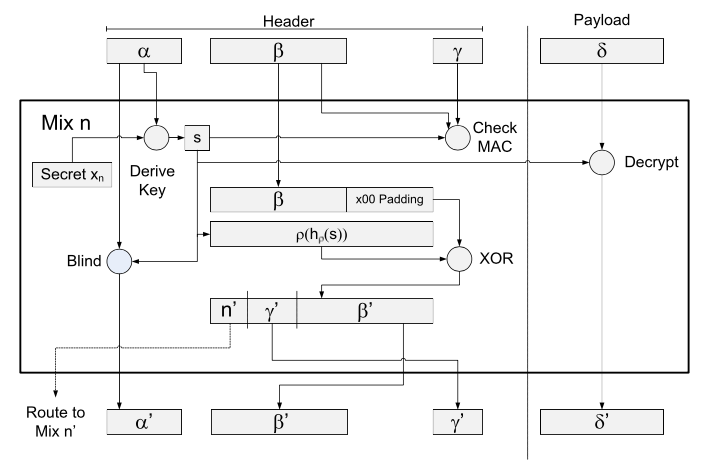
\includegraphics[width=12cm]{figs/sphinx.png}
    \caption{ How a sphinx message is processed at a node n. Source: \cite{danezis2009sphinx}}
    \label{fig:sphinx}
\end{figure}

\noindent
Here is how a node processes of a sphinx message $((\alpha, \beta, \gamma)\delta)$ as shown in fig.\ref{fig:sphinx}:\\
The $\alpha$ group element is used to derive a shared key $s$ using the nodes private key $x_n$ like this: $s = \alpha^{x_n}$.
These two and a hash function $h_b$ are used to blind the group element: $\alpha'= \alpha_i^{h_b(a,s)}$.
This blinded group element $\alpha'$ is used in the header for the outgoing message to the next node.
The integrity of the $\beta$ data is verified using the MAC $\gamma$ and the shared key $s$.
After it has been integrity checked the $\beta$ is decrypted using the shared key $s$ which reveals the routing information to the next node, and also $\beta'$ and $\gamma$ data for the next node. 
The payload $\delta$ is also decrypted into $\delta'$ using the key $s$, and used in the output message.
The final output message which is sent to the new node is $((\alpha', \beta', \gamma')\delta')$.

Here is how a node processes of a sphinx message $((\alpha, \beta, \gamma)\delta)$ as shown in fig.\ref{fig:sphinx}:\\
The $\alpha$ group element is used to derive a shared key $s$ using the nodes private key $x_n$ like this: $s = \alpha^{x_n}$.
These two and a hash function $h_b$ are used to blind the group element: $\alpha'= \alpha_i^{h_b(a,s)}$.
This blinded group element $\alpha'$ is used in the header for the outgoing message to the next node.
The integrity of the $\beta$ data is verified using the MAC $\gamma$ and the shared key $s$.
After it has been integrity checked the $\beta$ is decrypted using the shared key $s$ which reveals the routing information to the next node, and also $\beta'$ and $\gamma$ data for the next node. 
The payload $\delta$ is also decrypted into $\delta'$ using the key $s$, and used in the output message.
The final output message which is sent to the new node is $((\alpha', \beta', \gamma')\delta')$.


%\chapter{Project description evaluation criteria}


\bibliographystyle{plain}
%\bibliographystyle{gucmasterthesis}
\bibliography{imt4441}



\end{document}


IEEE computer society keywords
http://www.computer.org/portal/site/ieeecs/menuitem.c5efb9b8ade9096b8a9ca0108bcd45f3/index.jsp?&pName=ieeecs_level1&path=ieeecs/publications/author/keywords&file=ACMtaxonomy.xml&xsl=generic.xsl&
